\begin{figure}[h!]
    \centering
    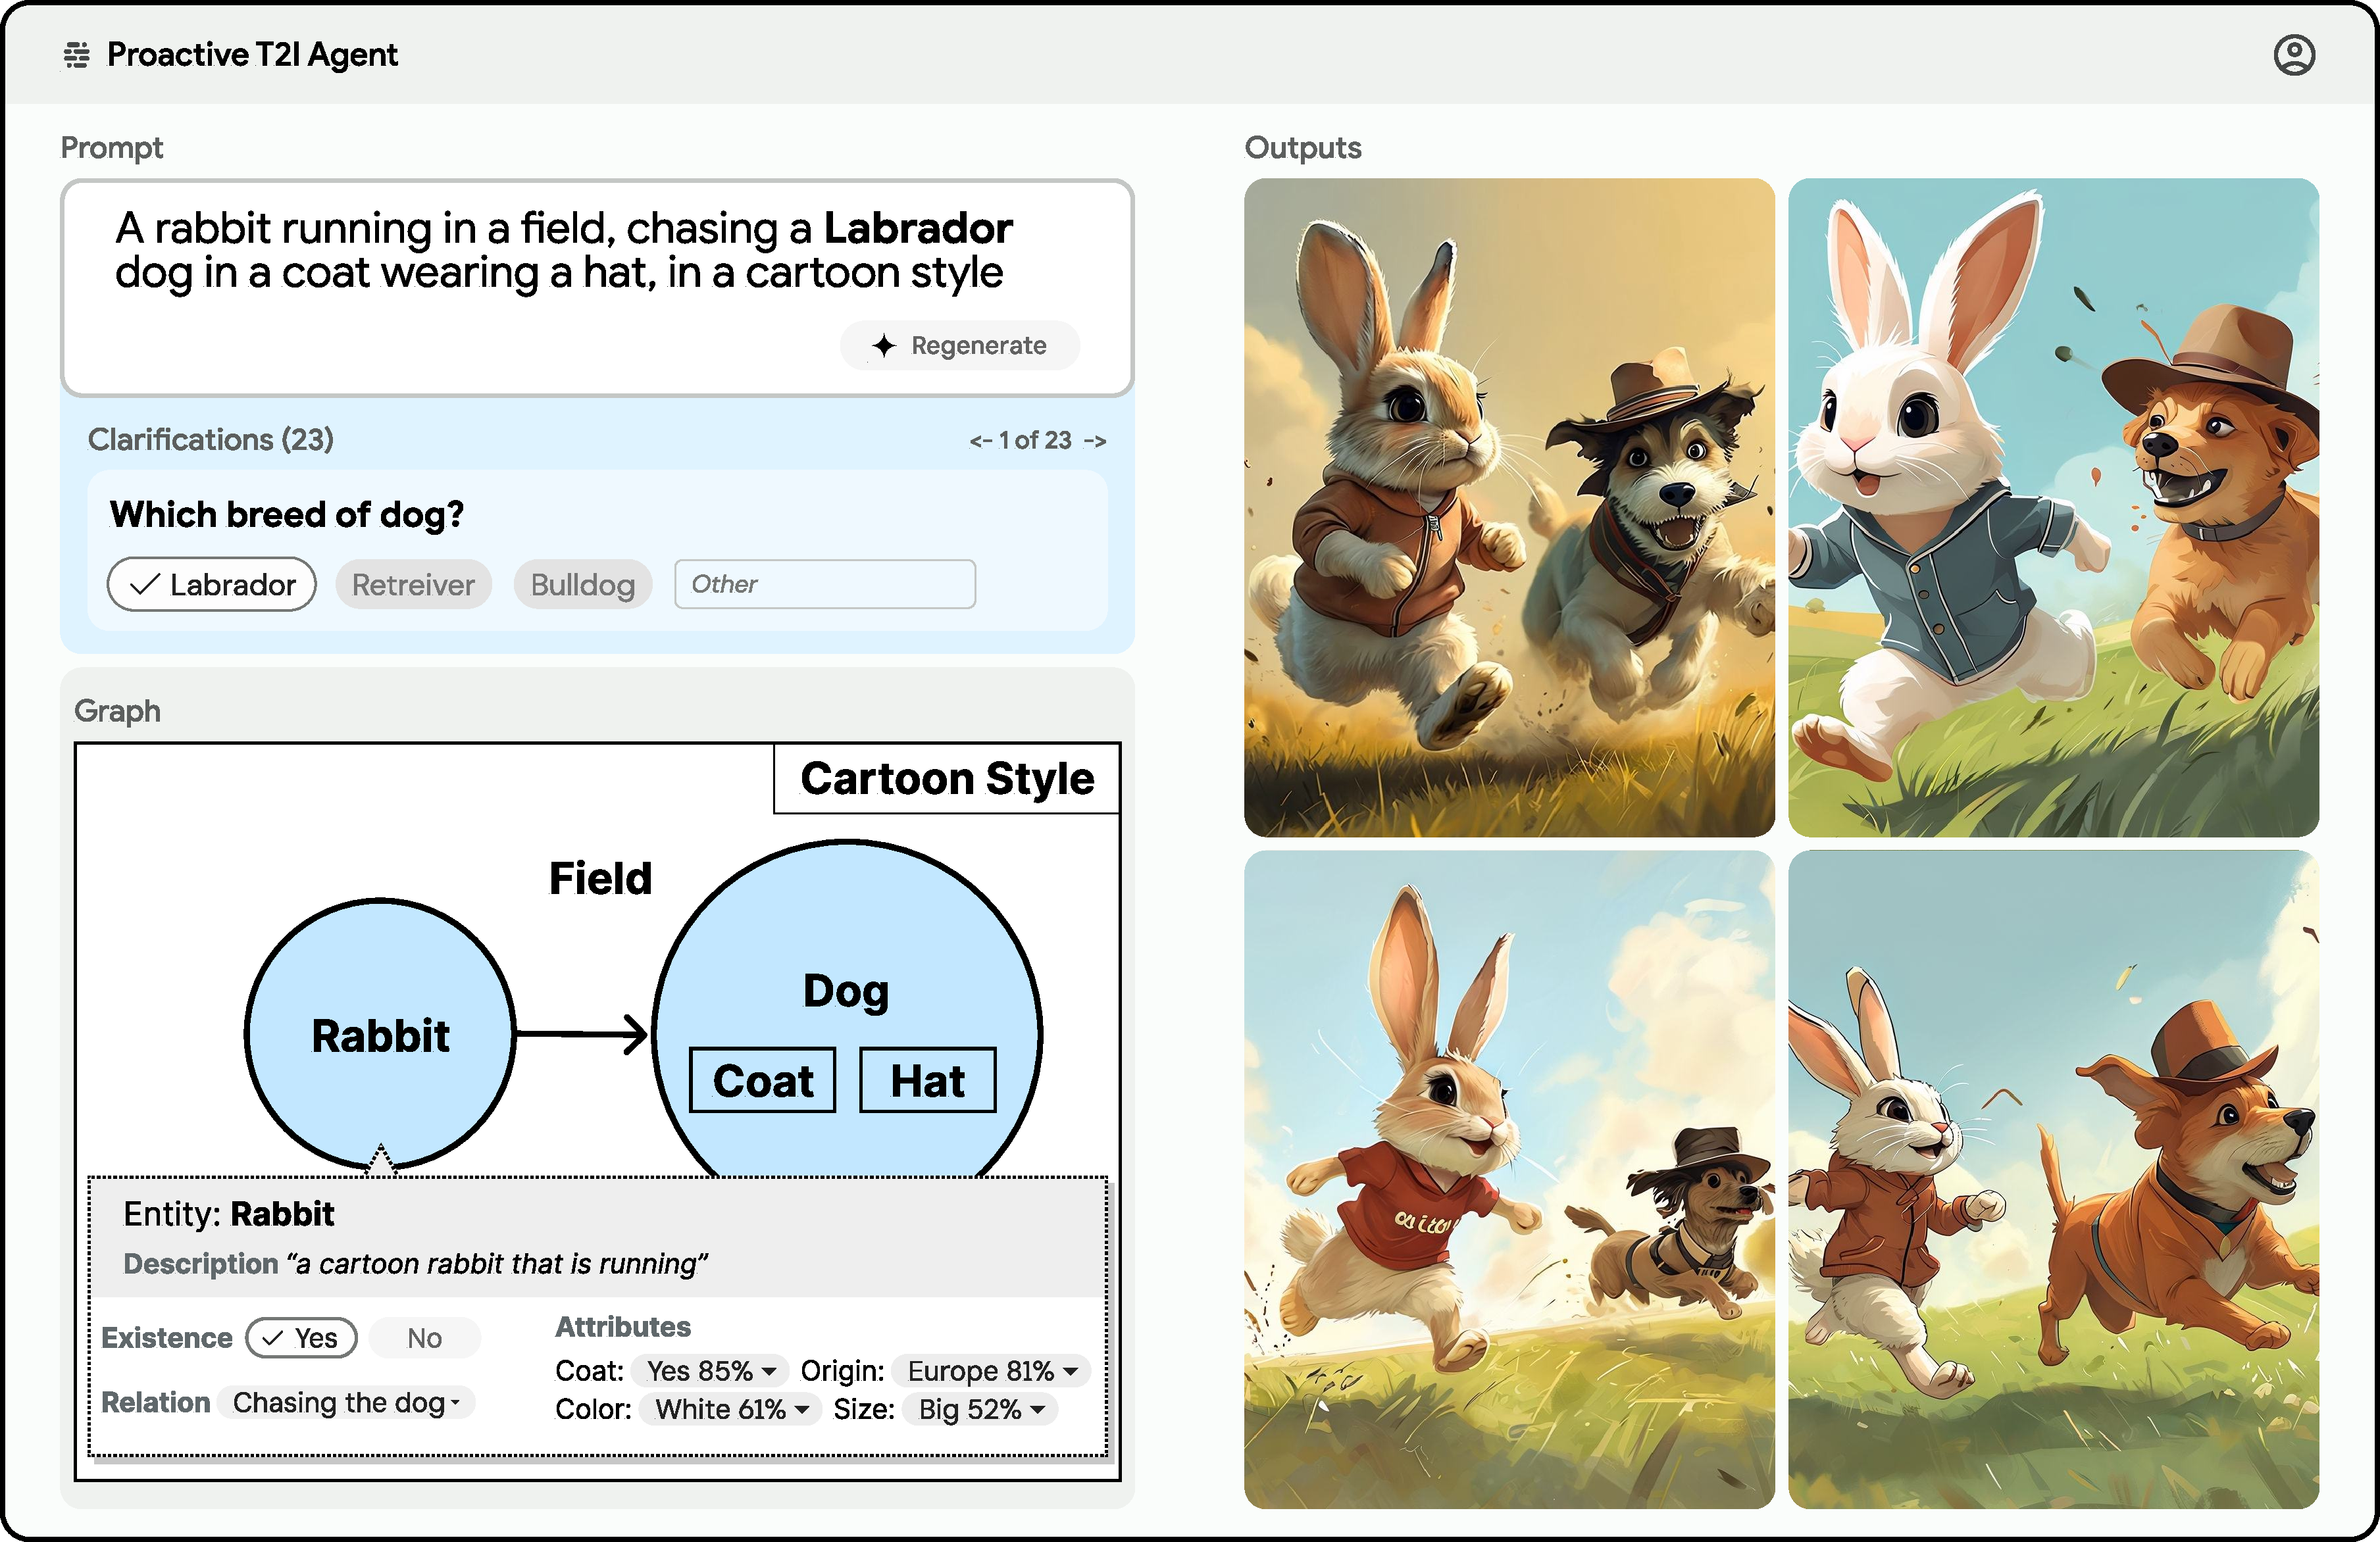
\includegraphics[width=.95\linewidth]{figures/Fig1.pdf}
    \caption{A proactive text-to-image agent interface that clarifies prompts, updates them based on user responses, and expresses its uncertainty and understanding as an editable belief graph.} %
    \label{fig:first_figure_interface}
\end{figure} 

\section{Introduction}
A fundamental challenge in the development of AI agents is how to foster effective and efficient multi-turn communication and collaboration with human users to achieve user-defined goals, especially when faced with the common issue of vague or incomplete instructions from humans. We focus specifically on text-to-image (T2I) generation, where recent advancements~\citep{imagenteamgoogle2024imagen3, betker2023improving, podell2023sdxl, yu2023scaling} have enabled the creation of stunning images from complex text descriptions. However, users often struggle to describe the image they would like to generate in a way that T2I systems can fully understand. This leads to unsatisfactory results and repeated iterations of prompts. %

The prompt underspecification problem arises from the inherent ambiguity of natural language, the different assumptions that humans make and the vast space of potential images that can be generated from a single prompt~\citep{hutchinson2022underspecificationscenedescriptiontodepictiontasks}. Imagine a prompt \textit{generate an image of a rabbit next to a cat}. This seemingly simple prompt leaves many important aspects underspecified: \textit{What kind of rabbit? What color is the cat? What is their relative positions? What is the background?} While a T2I model can generate an image with a rabbit and a cat in it, it is unlikely that the image captures the specific details a specific user has in mind. For example, people in Holland might assume it is common for rabbits to have lop ears, but people in New England might expect to see a cottontail rabbit with straight ears. The combination of all these factors can lead to a frustrating cycle of trial-and-error, with the user repeatedly refining their prompt in an attempt to steer the model towards the desired output~\citep{vodrahalli2023artwhisperer,huang2024dialoggen, sun2023dsg}. 

Instead of relying on passive T2I models that simply generate images based on potentially vague user instructions, we pursue a quest for agency in T2I generation. %
The T2I agents should actively engage with human users to provide a collaborative and interactive experience for image creation. We envision that these T2I agents will be able to (1) express and visualize their beliefs and uncertainty about user intents, (2) allow human users to directly control their beliefs beyond just text descriptions, and (3) proactively seek clarification from the human user to iteratively align their understanding with what the human user intends to generate.

In this work, we develop simple prototypes of such agents. At the core of those agent prototypes, we build in a graph-based symbolic belief state, named \emph{belief graph}, for agents to understand its own uncertainty about possible entities (e.g., rabbit) that might appear in the image, attributes of entities (e.g., rabbit's color), relations between entities and so on. Given a user prompt, we use an LLM and constrain its generation to the graph structure of beliefs, which include probability estimates on the appearance of entities and the possible values for attributes and relations. \Cref{fig:first_figure_interface} illustrates the interface and features of the prototypes. In particular, the agent can ask questions based on its uncertainty. For example, a very simple strategy is to find the most uncertain attribute of an entity (e.g., rabbit's color) and use an LLM to phrase a question about the attribute (e.g., What is the color of the rabbit?). The agent can also guide users to directly edit uncertain items in the graph. 

Based on user answers to agent questions or direct edits in the belief graph, the agent uses an LLM to update the prompt. It also transitions to a new belief graph by modifying the uncertainty of items clarified by the user. Based on the updated prompt, the agent calls an off-the-shelf T2I model to generate images. The structure of our agent prototypes is highly modular, making it easy to improve each component individually, e.g., changing the strategy for asking questions, updating the belief graph construction method, and switching to better LLMs or T2I models when they become available.


To evaluate the utility of our agent prototypes, we conduct both automatic evaluations and human studies.  We develop automatic evaluation pipelines to assess the effectiveness and efficiency of the T2I agents when interacting with simulated users with underspecified prompts answering questions based on their pre-fixed intents. The human studies aim to understand how helpful simple T2I agents can be and evaluate how good the agents' questions and generated images are.

We also create a hand-curated benchmark called DesignBench which contains aesthetic scenes with multiple entities and interactions between entities; it also contains both a short and long caption. DesignBench features diversity between photo-realism, animation and multiple styles allowing a robust testing with the use case of artists and designers in mind. 

We run automatic evaluations on DesignBench, the COCO dataset~\citep{lin2014microsoft} and ImageInWords \citep{garg2024imageinwordsunlockinghyperdetailedimage}.  Results show that our agents can achieve at least 2 times higher VQAScore~\citep{lin2024evaluatingtexttovisualgenerationimagetotext} than the traditional single-turn T2I generation within 5 turns of interaction. In our human study, over 90\% human subjects expect proactive clarifications to be helpful, about 85\% find belief graphs helpful, and 58\% think the question asking feature of agents could deliver value to their work very soon, or immediately. Participants prefer images generated by our simple agents over those of single-turn T2I systems in more than 80\% cases of the 550 prompt-image pairs used in the human study.

Our contributions: (1) the first explainable and controllable belief graph used for T2I, (2) novel design and prototypes for T2I agents that adaptively ask clarification questions and present belief graphs; (3) a new automatic evaluation pipeline with simulated users to assess question-asking skills of T2I agents; and (4) DesignBench: a new T2I agent benchmark.\footnote{Code and  DesignBench can be found at \url{https://github.com/google-deepmind/proactive_t2i_agents}.} \Cref{app:novelty} details the novelty.








